\chapter{Near infrared metrology of high performance silicon immersion gratings} 



\section{Introduction}
\label{sec:intro} 

Immersion gratings are diffraction gratings illuminated within a high refractive index optical material, which provides increased spectral resolving power compared to diffraction gratings of comparable size illuminated in air or vacuum.  Scientific demands for high spectral resolving power combined with engineering demands for compact spectrographs make immersion gratings an attractive technology.  This report chronicles the lab performance of CA1a, an immersion grating made of silicon ($n_{Si}\sim3.4$).  CA1a or its spare CA1b will serve as the primary dispersive optical element for the Immersion Grating Infrared Spectrometer, IGRINS\cite{yuk2010}.  We have reported on immersion grating design and fabrication elsewhere\cite{marsh2007}.  Wang et al. 2010\cite{wang2010} reported on the science requirements for, fabrication of, and optical testing results of CA1, the parent Si boule puck from which CA1a was cut.  Since 2010 we have cut and polished two optical devices from CA1, and report here on their performance \emph{in immersion}.

%%%%%%%%%%%%%%%%%%%%%%%%%%%%%%%%%%%%%%%%%%%%%%%%%%%%%%%%%%%%%
\section{Overview} 
Figure \ref{fig:CA1aphoto} shows a photo of the final immersion grating CA1a after cutting, polishing, AR coating, and aluminization.  The trapezoidal side profile is a relic from the shape of the parent substrate and our cutting strategy.  The optically active volume is the prism shown above the dashed line in the photo in Figure \ref{fig:CA1aphoto}.  We left on additional silicon to strengthen the thin end of the prism wedge.  The front entrance face has a multi-layer dielectric anti-reflection (AR) coating, which, based on direct measurements off the CA1a entrance face, has a reflectivity  $<1\%$ across the 1.4$-$2.5 $\mu$m range.  The grating grooves were aluminized with a conformal Al layer.  Cryogenic testing of heritage gratings demonstrated that the conformal layer of Al is robust to typical cryogenic thermal cycling\cite{marsh2007}. We have not yet cooled CA1a.

\begin{figure}
  \centering
  \subfloat[CA1a photo]{\label{fig:CA1aphoto}\includegraphics[height=5cm]{chSPIE_2012_CA1/figs/ca1_bartest2}}
	~
%  \subfloat[CA1a drawing]{\label{fig:CA1adraw}\includegraphics[page=1, trim=24cm 15.15cm 2cm 5cm, clip=true, totalheight=0.2\textheight ]{APRA_BOULE_29MM_R3_CA1_X14_2011-03-08}}
   \subfloat[CA1a drawing]{\label{fig:CA1adraw}\includegraphics[height=4cm]{chSPIE_2012_CA1/figs/ca1a_drawing}}
  \caption{Photo and design drawing of the immersion grating CA1a in the lab in August 2011.  The entrance face is on the right, with a light green color in the photo (color available in the digital manuscript), which is due to the AR coating.  The grating surface is on the top with microscopic grating lines perpendicular to the long edge of the grating.  In operation a 25 mm circular beam will be incident on the entrance face and will project into an ellipse on the grating surface as seen in the drawing.  The dispersed light will reemerge from the entrance face.  The units in the drawing are mm.  The parent substrate and grating geometry are pictured in Figures 1, 3, and 4 in Wang et al. 2010\cite{wang2010}.  Those figures reveal how the CA1a trapezoid shape and curved rear edge derive from the parent substrate shape.}
  \label{fig:gram}
\end{figure}

\begin{table}[h]
\caption {CA1 grating and substrate properties} \label{tab:title} 
\begin{center}
\begin{tabular}{lc}
\hline
Property & Value \\
\hline
Pitch, $\sigma$ ($\mu$m)  & 27.36 \\
$\;\;\;\;\;\;\;\;\;\;\;\;$(l/mm) & 36.55\\
Groove top, $t$ ($\mu$m)  & 9.95 \\
Blaze angle, $\delta$ ($^\circ$)  & 71.6$\pm$0.2 \\
Apex angle, $A$ ($^\circ$) & 72.1$\pm$0.2 \\
\multicolumn{2}{c}{\emph{Material properties}} \\
Material & High resistivity float zone Si \\
Average Refractive index & 3.44 \\
Specific heat ($J g^{-1} K^{-1}$) & 0.71 \\ 
\hline
\end{tabular}
\end{center}
\end{table}


We produce the grating grooves by photolithography and anisotropic chemical wet etching\cite{marsh2007, wang2010}.  This process has some special features.  The wet etching process makes acute angle grooves, not 90$^\circ$ grooves, as illustrated in Figure \ref{fig:CA1aSEM}.  The groove apex angle $A=70.5^\circ$ is the intersection of two 111 Si crystal planes.  We anticipated an apex angle widened by 0.8$^\circ$ on both sides, for a net apex angle of about $A=72.1^\circ$.  A finite but small amount of etching accross the 111 crystal planes causes the small 0.8$^\circ$ angular correction\cite[Figure 5]{marsh2007}.  The anisotropic correction similarly decreases the blaze angle $\delta$ by $\Delta \delta = 0.8^\circ$.  This effect must be accounted for, first at the time of the initial x-ray orientation and cutting of the parent substrate and second at the time of cutting the immersion prism from the Si parent substrate.  We verified the delivered blaze angle after wet etching but before cutting our immersion grating prism by measuring the relative intensity of eight diffracted orders in reflection in air at the air-Si grating interface.  We made a simple scalar diffraction theory model and compared it to the observed intensity of the eight orders surrounding order 82, the brightest observed order at 632.8 nm in front-surface reflection.  The measurements were performed in the Littrow configuration.  The model predicted the effect of the blaze envelope as a function of incidence angle.  We found $\delta=71.63\pm0.20^\circ$, consistent within the uncertainty with $\delta = R3$, so we cut the front face to R3.  The apex and blaze angles are conspicuous in the SEM cross section (Figure \ref{fig:CA1aSEM}).  Importantly, the groove apex shows a sharp peaked tip with no evidence of a flat bottom, which can occur in incomplete wet etching.  Flat bottoms cause a direct efficiency loss by diffracting light away from the blaze.  In the right panel of Figure \ref{fig:CA1aSEM} the optically active facets are highlighted.  The flat groove tops on the grating surface are artifacts of the groove formation process.  Specifically, nitride coated groove tops serve as anisotropic wet etch dams.  It is clear from the annotated SEM micrograph that the groove tops are shadowed for light incident at or close to the blaze angle.  The groove tops will be shadowed so long as the ratio of the grating top $t$ to pitch $\sigma$ ratio satisfies the condition:
\[ 
\frac{t}{\sigma} < \frac{1}{1+\frac{ \tan (A) }{ \tan (\delta{}) }}, 
 \] 
For our grating, $t/\sigma=0.36<0.49$, so the optically active groove facets fully shadow the groove tops as planned.  The SEM micrographs are not sensitive enough to small ($\sim5$ nm) scale groove position errors, so detailed optical and IR metrology is necessary to evaluate the performance.

%-------------
   \begin{figure}
   \begin{center}
   \begin{tabular}{c}
   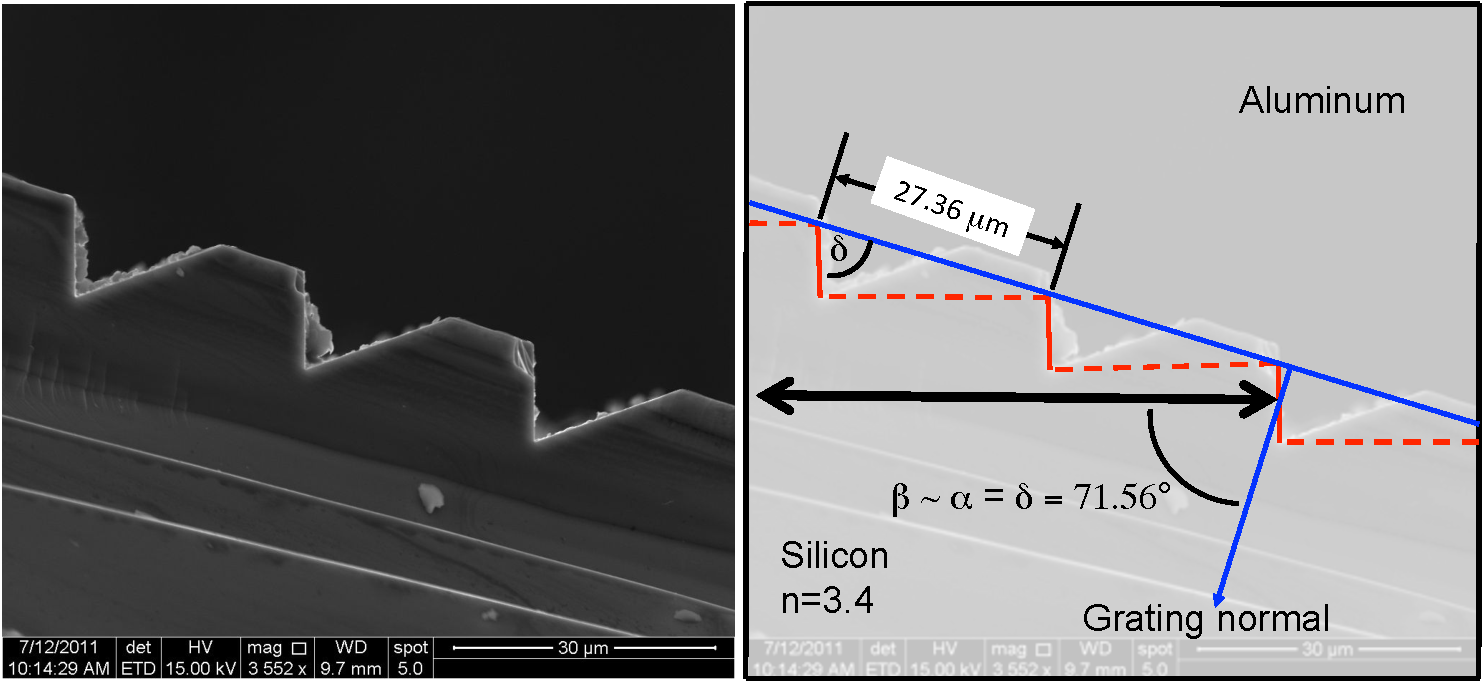
\includegraphics[height=7cm]{chSPIE_2012_CA1/figs/CA1_SEM_cross3}
   \end{tabular}
   \end{center}
   \caption[CA1a SEM]{ \label{fig:CA1aSEM}  Scanning electron micrograph (SEM) of a $\sim$100 $\mu$m cross section of a scrap portion of the immersion grating CA1.  The left panel is the unaltered SEM.  The right panel is a schematic illustrating the grating specifications and the geometry of incident and diffracted beams (thick black line with arrows).  The beam is incident from the left, and diffracts at the facets at the silicon/aluminum interface.  The incident angle $\alpha$ and diffracted beam $\beta$ are measured from the grating normal (shown in blue).  The blaze angle $\delta$ is set by the orientation of the crystal planes with respect to the grating surface.  This angle was designed to be $\delta=71.56^\circ$, which is the angle whose tangent is 3.  The optically active facets are highlighted as short red vertical lines (\emph{color online}).  The regions of the grating above the dashed line do not see the beam.  In the IGRINS design and in our lab testing there is a small out of plane angle $\gamma$ not shown here.  The apparent hillock artifacts on the grating facets are a result of the cross-section preparation process, the measured\cite{wang2010} surface flatness is 1.7 nm.}
   \end{figure} 
%-------------

\section{Efficiency} 
For optimal performance immersion gratings should be as efficient as possible.  The IGRINS specification for immersion grating efficiency is 65-70\% peak on blaze\cite{wang2010}. We directly measured the AR-coated entrance face reflective loss at $<1\%$ over the measured range $1500-2300$ nm.  From measurements of the microscopic surface roughness\cite{wang2010} we expect scattered light from microscopic surface roughness to be $<0.5\%$.  We directly measured the immersion grating efficiency as a function of wavelength with a custom scanning monochromator setup in our lab, described in the Section \ref{sec:GTA}.  The reference mirror was aluminum on glass, so the absolute grating efficiency is about 3.5\% lower than reported here, assuming aluminum reflectance of 95\% in the near-IR.  Recall that the grating grooves are aluminized, so the reported relative efficiency is a good indicator of how well the bulk of the immersion grating is performing.  The measurement shown in figure \ref{fig:CA1a-efficiency} has 1 nm bandwidth, with 1nm sampling over the range $1500-2300$ nm.  The measured peak on-blaze efficiency is between 70\% and 80\% across all 43 orders, except for order 120 which has a peak efficiency of 68\%.  CA1a was measured with an out of plane angle \cite{schroeder1987}, $\gamma \sim 2.6^\circ$ in immersion.  We only coarsely controlled the incidence angle $\alpha$ in our efficiency measurement, with $\alpha \sim \delta$ to within about 2$^\circ$.  Accordingly, we measured some angularly dependent diffraction loss that one would expect if orders diffracted into the grating sidewalls.  It is best to have $\alpha > \delta$ so that the blaze envelope is centered at $\beta < \delta$.


\begin{figure}
\begin{center}
 \begin{tabular}{c}
    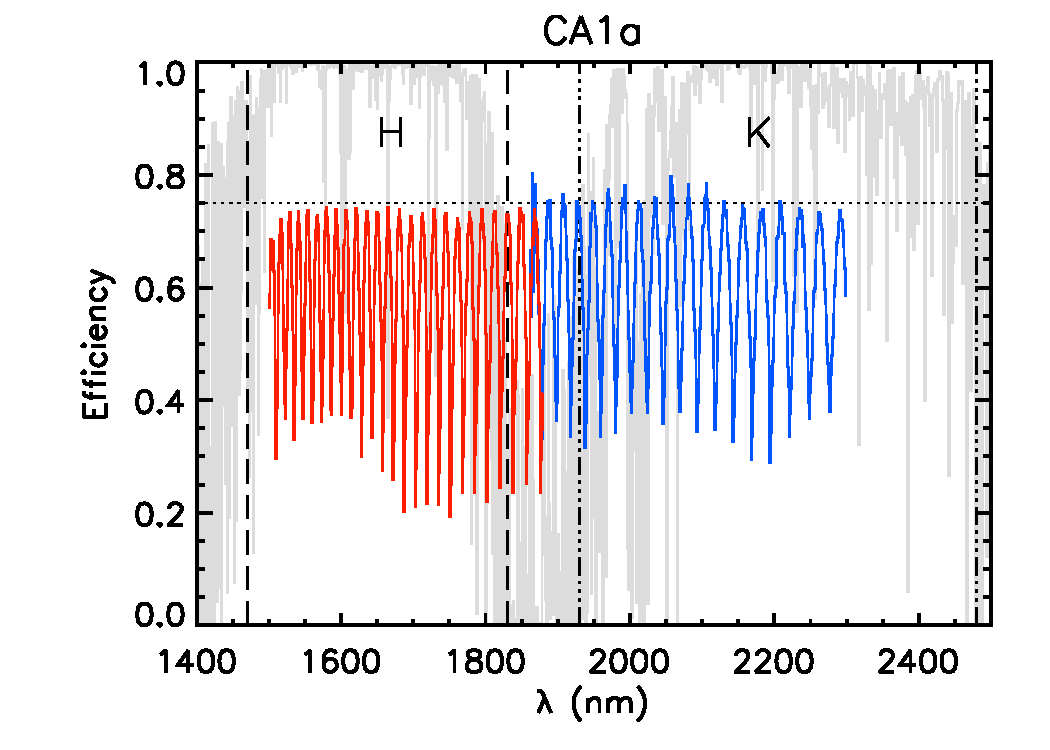
\includegraphics[width=1.0\textwidth]{chSPIE_2012_CA1/figs/CA1a_1500_2300_eff.pdf}
   \end{tabular}
  \end{center}
  \caption[CA1a Efficiency]{\label{fig:CA1a-efficiency} Efficiency of CA1a as a function of wavelength.  The measurements for 1500$-$2300 nm cover orders 120 to 78.  The peak on-blaze efficiency is typically about 75\% of an aluminum reference mirror, as shown by the horizontal dotted line at 75\%.  The vertical dashed lines at 1450 and 1900 nm demarcate the designed wavelength range of IGRINS $H-$band channel.  Similarly, the vertical dash triple-dotted lines demarcate the $K-$band channel.  The faint gray line in the background is the atmospheric transmission over Kitt Peak\cite{hinkle1995}.  Measurements at $\lambda > 2300 $ nm we not performed at the time of writing.  The slightly suppressed efficiency at 1500 nm may result from visible light leakage in the reference mirror measurement from our 1450 nm low pass filter operated in uncollimated light, or perhaps from real polarization sensitive effects.  See the notes on the next figure's caption regarding the difference in measurements shortward and longward of 1870 nm.}
\end{figure}

 There are a few potential loss mechanisms which lead to the observed efficiency:
\begin{enumerate}
\item Fresnel loss from entrance through the front vacuum/Si interface
\item Loss from microscopic groove and entrance face surface roughness that goes into scattered light
\item Loss at the Si/Al interface due to dielectric effects
\item Diffraction into other orders
\item Fresnel loss from exit through the front Si/vacuum interface
\item Systematic measurement error in beam alignment or collimation
\end{enumerate}

\section{Refractive index dependence}
The refractive index of silicon is wavelength and temperature dependent, so the blaze pattern in Figure \ref{fig:CA1a-efficiency} will be different at the cryogenic operating temperature of an IR spectrograph.  Precise measurements for crystalline Si are available for the CHARMS group at Goddard\cite{frey2006}.  The right panel of figure \ref{fig:CA1a-diffrac} shows the refractive index as a function of wavelength for 296 K, 273 K, and 77K, using the Sellmeier equation from the Goddard group and assuming vacuum wavelengths.  The index goes from about 3.483 to 3.445 in the wavelength range 1.5 to 2.3 $\mu$m, which is a change of about 1\%.  The index decreases by an average of 0.8\% from room temperature to 77K.  The index intimately controls both the diffraction angle $\beta$ at the Si-Al grating interface via the grating equation, and the refraction angle $\theta$ at the Si-vacuum interface via Snell's law.  For example the wavelength $\lambda=2.290 \;\mu$m at room temperature is diffracted to 78th order near the peak of the blaze.  Reducing the temperature to 77K decreases the index of refraction by 0.8\%. This puts $\lambda= 2.290 \;\mu $m into 77th order, which is at the edge of the blaze.  The grating period $\sigma$ also shrinks by a factor of the coefficient of thermal expansion (CTE) of Si, $\alpha \sim 3\times10^{-6}/^\circ$C.  From room temperature to 77K the fractional shrinkage is about 0.06\%, which is an order of magnitude less than the effect of the index of refraction.  Furthermore, the CTE effect will have no effect at the Si-vacuum interface.

\begin{figure}
\begin{center}
 \begin{tabular}{c}
    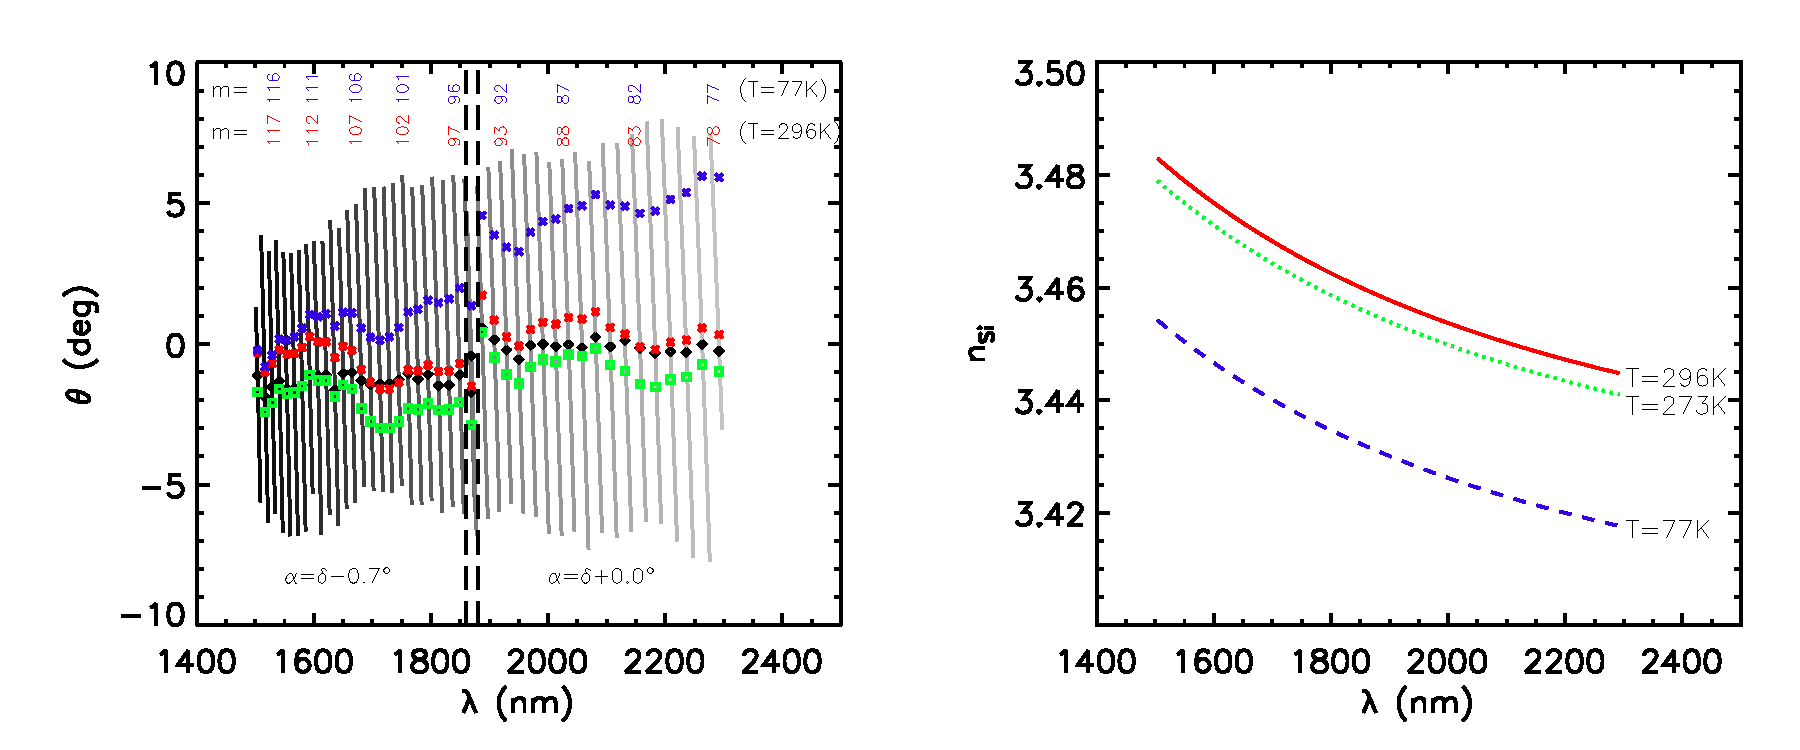
\includegraphics[width=1.0\textwidth]{chSPIE_2012_CA1/figs/CA1a_diffrac}
   \end{tabular}
  \end{center}
  \caption[CA1a Diffraction]{\label{fig:CA1a-diffrac} Measured and predicted diffraction angles for CA1a.  The right panel is the index of refraction as a function of wavelength\cite{frey2006} for T = 296, 273, and 77 K.  The left panel is the angular position of diffracted beams as a function of wavelength.  The almost vertical lines are approximately 1 free spectral range of the observed 43 diffraction orders for $1500 < \lambda (\textrm{nm}) < 2300$ in air at T = 296K.  The order numbers for every fifth order, starting at 78th order are marked at the top.  The black diamonds are the observed peaks of the blaze efficiency (cf. figure \ref{fig:CA1a-efficiency}).  The measurements longward and shortward of $\lambda=1870$ nm have slightly different incidence $\alpha$ angles, which jogged the the blaze center positions.  The red $\ast$, green square, and blue $\times$ demarcate the expected positions of beams from scalar optics diffraction and refraction theory assuming a Si refractive index at the temperatures of T=296, 273, and 77 K, respectively.  The model corrects for $\alpha \neq \delta$ measurements for $\lambda < 1870 $ nm, causing a jog in the $\theta(\lambda)$ trend highlighted by the vertical black dashed lines.  The temperature change shifts the position of diffracted beams by an entire order.}
\end{figure}

\section{Periodic errors, ghosts, and large scale performance} 

\begin{figure}
  \centering
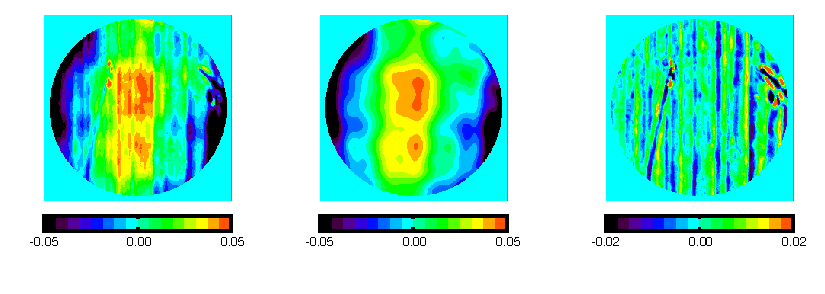
\includegraphics[width=0.9\textwidth]{chSPIE_2012_CA1/figs/CA1a_fig_scl2}
  \caption{Optical interferometry of CA1a in reflection off the back surface before cutting and aluminization.  The color scales are in waves of surface error for 632 nm in reflection.  \emph{Left:} Interferogram measured in Littrow reflection at R3 over a 23.75 mm beam on the parent substrate CA1, in the vicinity where CA1a was later cut.  The colorbars show the vertical scale in waves of surface distortion at $\lambda = $ 632.8 nm.  These optical measurements illuminate the back of the grating facets, they were taken before aluminization and should be a good proxy for immersion performance at 2.15 $\mu$m. \emph{Center:} A fit to the large scale surface distortion using the first 200 Zernike polynomials in the Noll Sequence \cite{noll1976}.  \emph{Right:} The residual high spatial frequency surface error constructed from subtracting the fit from the measured surface error.}
  \label{fig:gram}
\end{figure}

Figure \ref{fig:gram} shows the optical 632 nm interferogram of CA1 in reflection in air.  The peak to valley surface error is 0.17 waves.  These interferograms should be equivalent to 2.16 $\mu$m in immersion in a cryogenic environment.  The shortest operational wavelength for the IGRINS instrument is 1.45 $\mu$m, at which the surface error is 0.25 waves.  The surface structure can be broken into two components, the large scale surface aberration and and a periodic error of parallel stripes parallel to the grating grooves.  Figure \ref{fig:gram} shows the large scale surface aberration in the middle panel and the periodic error on the right panel.  The vertical stripes are conspicuous in the right panel, while the center panel looks like a typical residual optical surface aberration possessing relatively low amplitude.  The main power in the periodic error is in a single sine wave with 5 mm deprojected period and amplitude of 3.2 nm.  There are other harmonic components with higher spatial frequency and comparable or lower amplitude.  

The origin of the large scale surface aberration is a combination of the dozen or so processing steps that go into delivering the final immersion grating.  Chief among these is the UV contact photolithography step.  The reactive ion etching, wet etching, and surface preparation steps may also contribute to the overall surface error.  The periodic stripes arise in the UV photolithography process that transfers the pattern from the photomask to the underlying photoresist.  Specifically the contacted mask and Si substrate pair repeatedly translate beneath a 1 cm wide UV slit to deliver the requisite UV dose.  We discovered that the translation stage had a periodic speed change which is equivalent to a periodic exposure time as a function of position on the photoresist.  Prototype gratings made since CA1 have corrected for this problem and surface errors attributable to periodic errors have largely disappeared.  

The major problem with periodic errors is that they cause symmetric ghosts surrounding the main diffraction peak.  The intensity of the ghosts relative to the main peak is related to the periodic error amplitude by\cite{marsh2007, james2007, wang2010}:
\begin{eqnarray}
	\frac{I_{\textrm{ghost}}}{I_{\textrm{line}}}= \left \lbrack \frac{2\pi n}{\lambda} \xi \sin{\delta} \right \rbrack ^2
\end{eqnarray}
where $\xi$ is the amplitude of the spacing error.  Figure \ref{fig:PSFzygo} shows a logarithmically scaled PSF from optical interferometry of CA1a in reflection from the aluminized surface in air at 632.8 nm over a 25 mm circular aperture.  The measured intensity of the ghost relative to the main peak is $I_{g}/I_{0}=9\times10^{-4}$.  Optical spectral purity lab measurements at 632.8 nm are higher by 20\%.  Measurements at 543 nm (comparable to 1.87 $\mu$m in immersion), show a level of $I_{g}/I_{0}=1.6\times10^{-3}$, which is 30\% greater than one would expect from scaling interferometrically derived intensity at 632.8 nm.  Extrapolating the interferometrically derived intensity to 1.45 $\mu$m in immersion, the ghosts in IGRINS will have a peak intensity of 0.2\% of the main peak.  Quantitative lab measurements at 1.523 $\mu$m in immersion were attempted but were not reliable due to nonlinear response at the requisite high dynamic ranges need to measure the low ghost levels.  

\begin{figure}
\begin{center}
 \subfloat[2D Zygo PSF]{\label{fig:zygoPSF2D} 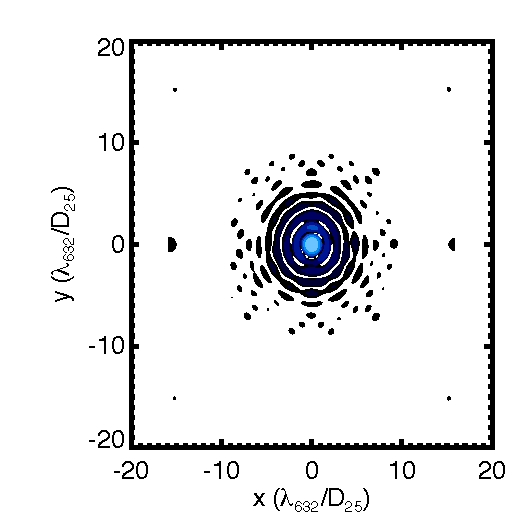
\includegraphics[width=0.45\textwidth]{chSPIE_2012_CA1/figs/CA1a_ghost_zygo_2d}}
 \subfloat[1D Log PSF]{\label{fig:logPSF1D} 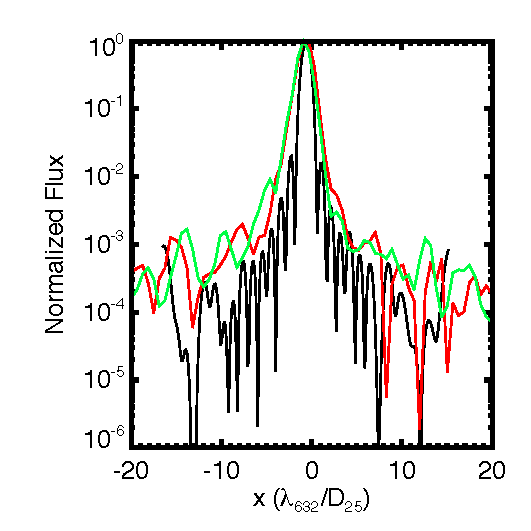
\includegraphics[width=0.45\textwidth]{chSPIE_2012_CA1/figs/CA1a_ghost_1d}}   
  \end{center}
  \caption[Immersion grating interferogram PSF]{\label{fig:PSFzygo}  Left: The 2-dimensional synthetic PSF from interferometric measurements of the air-aluminum reflective interface of CA1a at 632.8 nm at R3.  The dispersion direction is $x$, the cross-dispersion or spatial dimension is $y$.  The units on the axes are in terms of diffraction widths of $\lambda=$ 632.8 nm and $D=$ 25 mm, which were the conditions of the interferometry.  The scale on the 2D image is linear, compare to the intensity levels shown on the right panel.  Right:  The 1D logarithmically scaled horizontal line profile of the PSF of CA1a under three conditions.  The black is the synthetic interferometric PSF.  The red is the lab-measured PSF in reflection at 632 nm with a 20 mm beam.  This measurement is not diffraction limited.  The green line is the measurement at 543 nm in reflection with a 20 mm beam.}
\end{figure}


\section{Measurement setup description} \label{sec:GTA}
The basic strategy of the custom efficiency measurement setup is to compare the chopped signal from the immersion grating to an aluminum mirror.  The monochromator outputs 1 nm bandwidth and we sample at 1 nm steps.  The basic layout is a light source, 1.45 $\mu$m long pass filter, Spectral Products DK480 scanning monochromator, a chopper, collimating and relay optics, a motorized swing arm, a single pixel PbS array, and a lock-in amplifier.  The DK480, motorized swing arm, and lock-in amplifier are all computer controlled.  Custom software predicts the diffraction angles of the immersion grating and fine scans the swing arm around the predicted angular order positions.  Figure \ref{fig:GTAview} shows a labelled photo of the measurement apparatus, with detailed description of the optical path in the figure caption.  

\begin{figure}
\begin{center}
    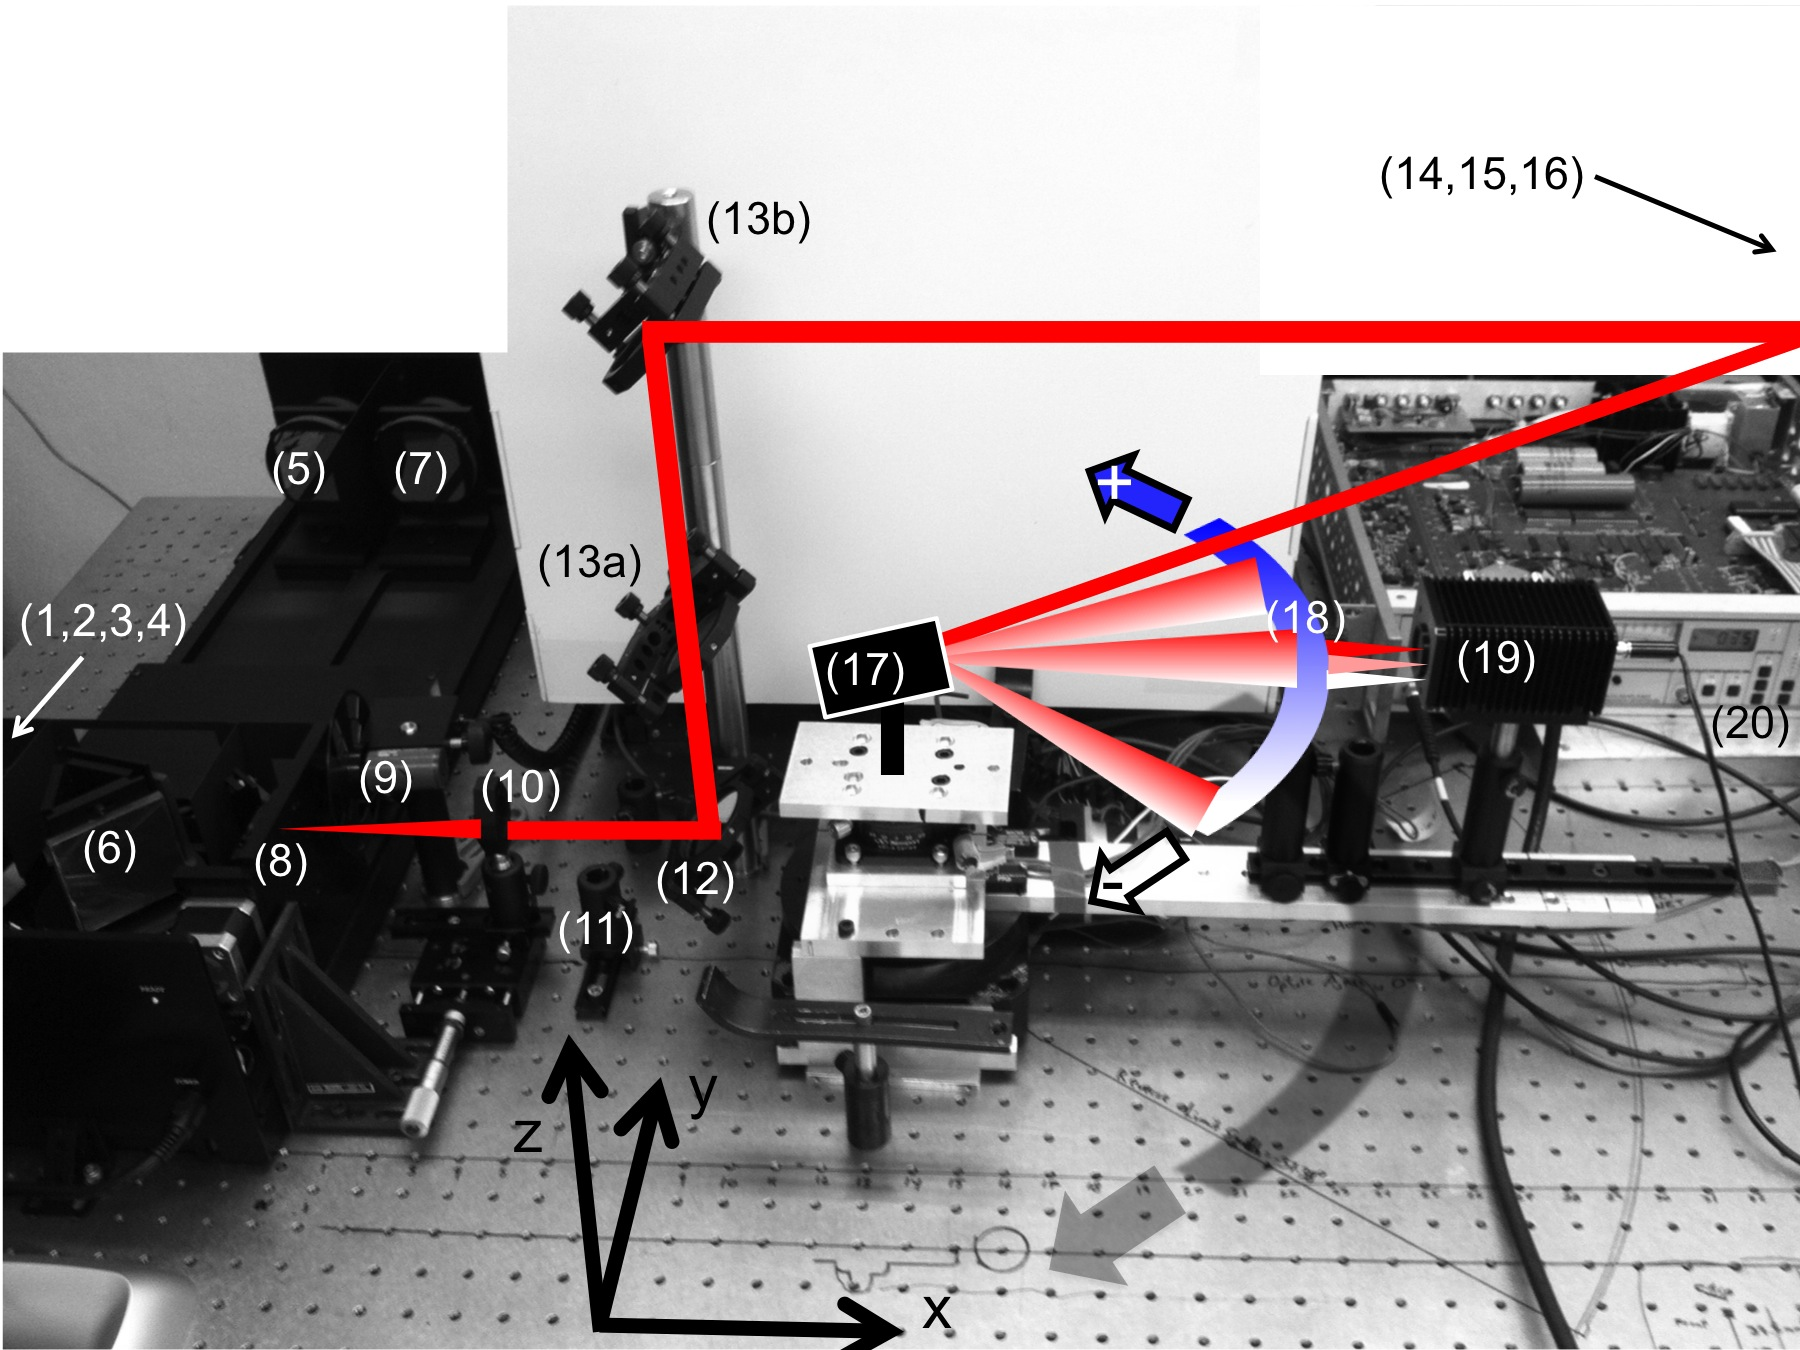
\includegraphics[width=1.0\textwidth]{chSPIE_2012_CA1/figs/GTA_cam_model_ref_tilt.jpg}
  \end{center}
  \caption[View of the monochromator, periscope, and swing arm-camera system with the beam path highlighted]{\label{fig:GTAview} View of the monochromator, periscope, and swing arm-camera system with the beam path highlighted.  The beam exits the monochromator exit slit (8), where the optical chopper (9) is located.  The beam is collimated by a 1 inch post-slit lens (10).  The periscope system includes 3 mirrors (12, 13a, 13b), only two of which are active at any time.  In the reflective arm of interest to this report, we use mirrors (12) and (13b), with mirror 13a moved clear out of the beam path with a 90$^\circ$ flip mount.  The beam travels about 1 meter (off the image) to an adjustable iris in double pass (14, 16) sandwiching a mirror (15) tilted about 10$^\circ$ from the $z-y$ plane.  The beam travels along the vector terminating on the center of the immersion grating (17).  The immersion grating has its grooves vertical (parallel to the $z-$axis) so that the dispersion occurs in a the $x-y$ plane.  There are typically 3 or 4 orders diffracted $\pm20^\circ$ from the optical axis, for CA1 in our wavelength range of interest ($1.5-2.5 \; \mu$m).  The camera lens (18) and single pixel detector (19) are mounted on a swinging arm which rotates in the $x-y$ plane, with its center of rotation equal to the position of the immersion grating.  The angular range of motion of the swing arm is about +27 to -37$^\circ$ which is set by limit switches and the rigid mechanical structure, which supports the immersion grating and its concomitant fine adjust positioning hardware.  The cartoon arrows demonstrate our angular sign convention which is positive counter clockwise, with zero along the optic axis.  The grating normal is at about -70$^\circ$ with that convention.  The beam path in the monochromator is omitted for clarity.  The lock-in amplifier electronics are marked with number (20).}
\end{figure}

